\chapter{Implementierung} % (fold)
\label{sec:implementierung}
Nachfolgend soll die Implementierung der verschiedenen APIs, sowie die Grundprinzipien während der Implementierung, beschrieben werden.
\section{Grundprinzipien während der Implementierung} % (fold)
\label{sec:prinzipien}
Im Rahmen der Implementierung dieser Anwendung wurden verschiedene Grundprinzipien beachtet, die sowohl die Qualität als auch die Erweiterbarkeit der Anwendungen  sicherstellen. Die Wahl der verwendeten Technologien sowie die Anwendung bewährter Praktiken standen dabei im Vordergrund. Als Basis für die Entwicklung wurde Java JDK 17.0.10 Corretto gewählt, da diese Version eine Long-Term-Support (LTS)-Version darstellt und damit eine stabile und sichere Grundlage für die Entwicklung bietet. Amazon Corretto bietet eine optimierte JVM, wodurch alle Softwarebestandteile auf jeder Plattform mit einer zertifizierten JAVA Virtual Machine lauffähig sind. Ergänzt wurde das JDK durch Spring Boot Version 3.3.4, eine weit verbreitete Plattform für die Entwicklung von Webanwendungen und Microservices. Spring Boot ermöglicht eine schnelle und einfache Konfiguration von Anwendungen und vereinfacht den Entwicklungsprozess durch das Automatisieren von häufig auftretenden Aufgaben, wie etwa der Konfiguration von Servern und Datenbankverbindungen.

Ein zentrales Konzept während der Implementierung war die Verwendung von Dependency Injection. Diese Technik sorgt dafür, dass die Abhängigkeiten zwischen den einzelnen Komponenten der Anwendung nicht hart kodiert sind, sondern zur Laufzeit durch den DI-Container von Spring injiziert werden. DI fördert die Entkopplung von Komponenten, was zu einer besseren Testbarkeit, Flexibilität und Wartbarkeit des Codes führt. Da der Code durch DI in unabhängige, gut getestete Module unterteilt wird, lässt er sich leicht erweitern und an geänderte Anforderungen anpassen. Zudem trägt DI zur Verbesserung der Lesbarkeit des Codes bei, da Abhängigkeiten nicht explizit im Konstruktor oder an anderen Stellen erstellt werden müssen.

Die Implementierung der Anwendung erfolgte unter der Berücksichtigung von Best Practices, die die Qualität des Codes sicherstellen und eine effiziente, langfristige Wartung ermöglichen. Ein wesentlicher Aspekt war hierbei die Modularität der Lösung. Die Anwendung wurde so strukturiert, dass jede Komponente eine klare, abgegrenzte Verantwortung übernimmt. Dies sorgt nicht nur für eine bessere Nachvollziehbarkeit des Codes, sondern erleichtert auch das Testen und die Erweiterung von Funktionalitäten. Bestehende Komponenten können so problemlos durch neue ersetzt oder erweitert werden, ohne die gesamte Anwendung zu beeinträchtigen.




% section prinzipien (end)

\section{Post REST} % (fold)
\label{sec:postrest}
In dieser Arbeit steht "PostREST" für die PostgreSQL REST-API, die eine Schnittstelle für den Zugriff auf eine PostgreSQL-Datenbank über HTTP-Anfragen bietet. Diese API implementiert eine Reihe von Endpunkten, die in Abschnitt 5.2.1 der Arbeit definiert sind. Diese Endpunkte sind dafür verantwortlich, bestimmte Anfragen zu bearbeiten und entsprechende Antworten zurückzugeben.
\noindent
Die zentrale Komponente, die dafür sorgt, dass die Endpunkte korrekt verarbeitet werden, ist die Controller-Klasse. In dieser Klasse sind die Endpunkte integriert, wobei jeder Endpunkt mit seinen spezifischen Pfadvariablen und den Rückgabewerten versehen ist. Die Controller-Klasse übernimmt die Aufgabe, die richtigen Methoden auszuführen, wenn eine Anfrage an einen bestimmten Endpunkt gestellt wird.
\noindent
Der PostrestController ist die konkrete Implementierung des Controllers, der die Geschäftslogik verarbeitet. Er ruft den DBService auf, welcher das Interface IDBService implementiert. Das Interface definiert die Methoden, die notwendig sind, um Daten aus den zugrunde liegenden Datenbanken abzurufen. Diese Methoden kapseln die Logik für den Datenbankzugriff und sind so gestaltet, dass sie von der Controller-Klasse verwendet werden können, um die richtigen Informationen zu erhalten.
\noindent
Die Kommunikation zwischen den verschiedenen Schichten der Anwendung erfolgt durch Dependency Injection. Das bedeutet, dass die verschiedenen Komponenten nicht direkt in der Controller-Klasse erzeugt werden, sondern von außen in die Klasse injiziert werden. In diesem Fall werden die Repositorys der verschiedenen Entitäten in die Controller-Klasse injiziert. Diese Repositorys sind verantwortlich für den direkten Datenbankzugriff und beinhalten die notwendigen Methoden und SQL-Abfragen, die zum Abrufen und Verwalten der Daten in der Datenbank erforderlich sind.
\noindent
Nachdem die Daten erfolgreich aus der Datenbank abgefragt wurden, werden sie durch die Hierarchie der Anwendung weitergegeben. Der PostrestController sorgt dafür, dass die abgerufenen Daten in das gewünschte Format für die API-Antwort umgewandelt werden. Dies ist in diesem Fall das JSON-Format, dass dann dem Nutzer der API als Antwort übermittelt wird. Diese Antwort enthält die angeforderten Informationen, die der Nutzer über die API abgefragt hat.
\begin{figure}[H]
	\centering
	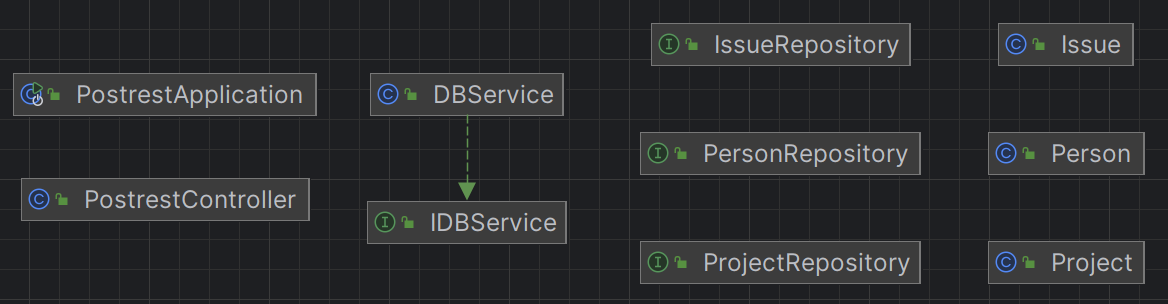
\includegraphics[scale=0.5]{Illustrations/postrest.png}
	\caption{Java Klassen PostREST}
\end{figure}

% section postrest (end)

\section{Post Graph} % (fold)
\label{sec:postgraph}
Hierbei handelt es sich um eine GraphQL API mit PostgreSQL Datenbank. 
\begin{figure}[H]
	\centering
	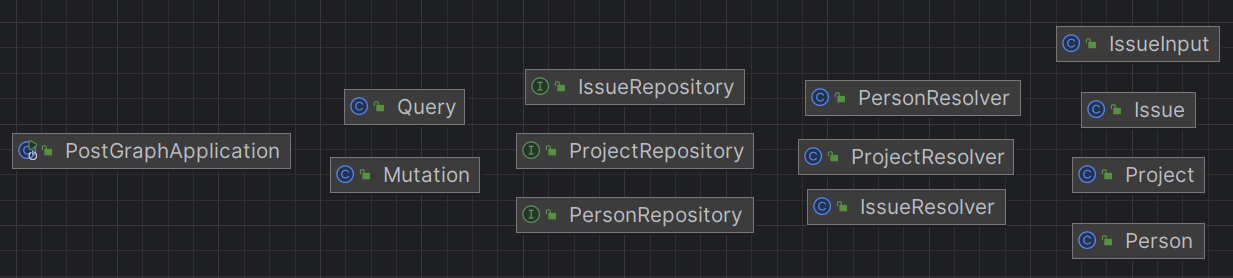
\includegraphics[scale=0.5]{Illustrations/postgraph.png}
	\caption{Java Klassen PostGraph}
\end{figure}
% section postgraph (end)

\section{Neo4REST} % (fold)
\label{sec:neo4rest}
\begin{figure}[H]
	\centering
	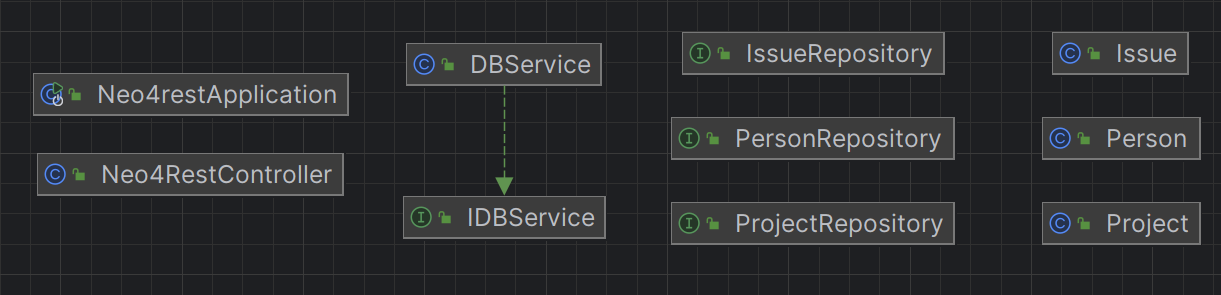
\includegraphics[scale=0.5]{Illustrations/neo4rest.png}
	\caption{Java Klassen Neo4REST}
\end{figure}
% section neo4rest (end)

\section{Neo4Graph} % (fold)
\label{sec:neo4graph}
\begin{figure}[H]
	\centering
	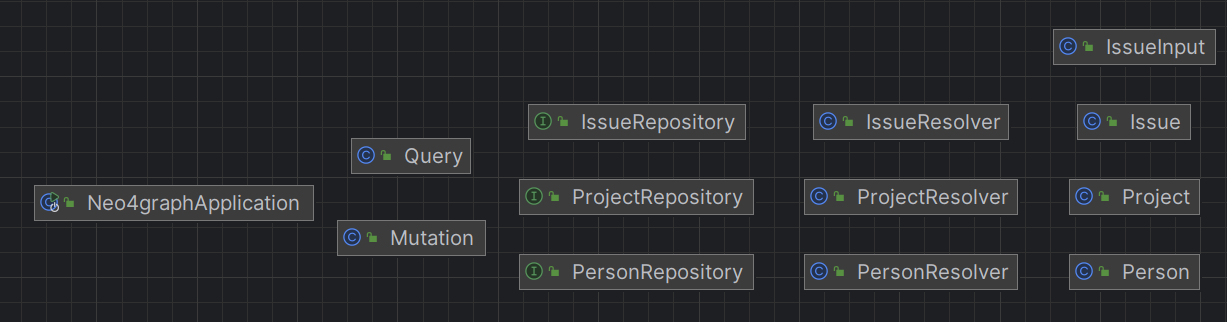
\includegraphics[scale=0.5]{Illustrations/neo4graph.png}
	\caption{Java Klassen Neo4Graph}
\end{figure}
% section neo4graph (end)


% chapter implementierung (end)